\section{Consensus layer support} \label{sec.consensus}

\subsection{The interlink pointers data structure}
\label{sec.interlink}

We will now start constructing a concrete blockchain proof protocol. Before
we're able to define the prover and the verifier algorithms, we need to propose
certain modifications to the consensus layer.

We now observe that some blocks will achieve a much lower id. Observe then that
in expectation, half of the blocks will be of level $1$, $1/4$ of the blocks
will be of level $2$, $1/8$ will be of level $3$ and $1/2^\mu$ blocks will be of
level $\mu$. In expectation, the number of superblock levels of a chain $\chain$
will be $\log(\chain)$.

Figure~\ref{fig.hierarchy} illustrates the blockchain superblocks starting from
level $1$ and going up to level $4$ in case these blocks are distributed
exactly according to expectation. Note that each level contains half the blocks
of the level below.

\begin{figure}
    \caption{The hierarchical blockchain.
    Higher levels have achieved a lower target (higher difficulty) during mining.}
    \centering
    \iftwocolumn
        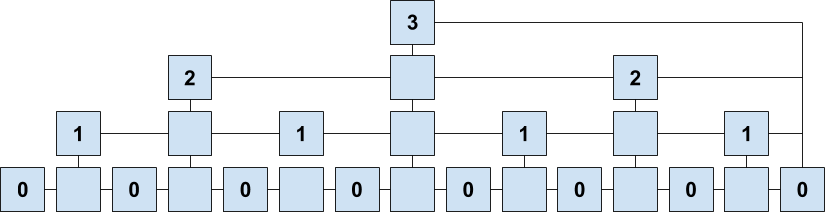
\includegraphics[width=\columnwidth,keepaspectratio]{figures/hierarchical-ledger.png}
    \else
        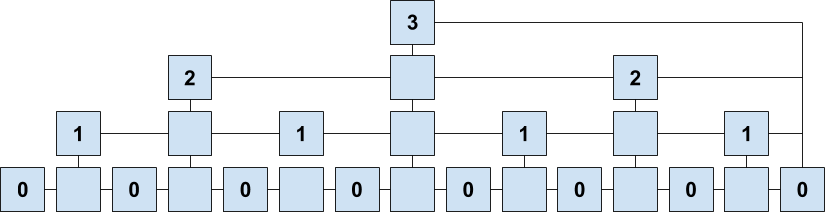
\includegraphics[width=0.7\columnwidth,keepaspectratio]{figures/hierarchical-ledger.png}
    \fi
    \label{fig.hierarchy}
\end{figure}

The \textit{interlink} data structure is proposed to be included in each block,
replacing the existing pointer to the previous block with a list of pointers to
a small number of previous blocks. For each superblock level $\mu$, this data
structure contains a pointer to the most recent preceding block of level $\mu$.
The algorithm for this construction is shown in
Algorithm~\ref{alg.nipopow-interlink} and is borrowed from \cite{KLS}. Genesis
is of infinite level and hence a pointer to it is included in every block at the
first available index within the interlink data structure. The interlink data
structure turns the blockchain into a skiplist-like data structure. Observe that
the number of pointers that need to be included per block, in expectation, is
$\log(\chain)$.

The updateInterlink algorithm accepts a block $B'$, which already has an
interlink data structure defined on it. The function then evaluates the
interlink data structure which needs to be included as part of the next block.
The algorithm proceeds by copying the existing interlink data structure and
then modifying some of its entries from level $0$ to the level of block $B'$ to
point to the block $B'$. Observe that the pointers stored are block ids and
hence block data needs to be looked up based on blockid. To this end, the full
node maintains a \textit{blockbyid} dictionary which, queried with the block
id, returns the block data. Finally, the full node also maintains a
\textit{depth} data structure which, given a block, returns its distance from
the Genesis block.

% \import{./}{algorithms/alg.nipopow-helper.tex}
\import{./}{algorithms/alg.nipopow-interlink.tex}

\subsection{Superchain quality}

We now formally describe the distribution of superblocks within a blockchain.

\begin{definition}[Locally good superchain]
A superchain $\chain'$ of level
$\mu$ with underlying chain $\chain$ is said to be $\mu$-\textnormal{locally-good}
with respect to security parameter $\delta$, written
$\textsf{local-good}_{\delta}(\chain', \chain, \mu)$, if $|\chain'| > (1 -
\delta)2^{-\mu}|\chain|$.
\end{definition}

\begin{lemma}[Local goodness]\label{lem.localgood}
Assume chain $\chain$ contains only honestly-generated blocks and has been
adopted by an honest party in an execution with random network scheduling. Then
for all levels $\mu$, for all constant $\delta > 0$, all continuous subchains
$\chain' = \chain[i:j]$ with $|\chain'| \geq m$ are locally good,
$\textsf{local-good}_{\delta}(\chain', \chain, \mu)$, with overwhelming
probability in $m$.
\end{lemma}
\begin{proof} \textbf{(Sketch)}
Observing that for each honestly generated block the probability of being a
$\mu$-superblock for any level $\mu$ follows an independent Bernoulli
distribution, we can apply a Chernoff bound to show that the number of
superblocks within a chain will be close to its expectation, which is what
is required for local goodness.
% \dznote{Articular the exact Chernoff bound here}
\qed
\end{proof}

\begin{definition}[Chain superquality]
The $(\delta, m)$ superquality property
$Q^\mu_{scq}$ of a chain $\chain$ pertaining to level $\mu$ with security
parameters $\delta \in \mathbb{R}$ and $m \in \mathbb{N}$ states that for all
$m' \geq m$, it holds that $\textsf{local-good}_{\delta}(C\upchain^\mu[-m':],
C\upchain^\mu[-m':]\downchain, \mu)$. That is, all suffixes that are
sufficiently large are locally good.
\end{definition}

\begin{lemma}[Superquality]\label{lem.superquality}
For all levels $\mu$, for all constant $\delta > 0$, a chain
$\chain$ containing only honestly-generated blocks adopted by an honest party in
an execution with random network scheduling has $(\delta, m)$-superquality at level
$\mu$ with overwhelming probability in $m$.
\end{lemma}

\begin{proof}
Let $\chain' = \chain\upchain^\mu$ and let $\chain^* =
\chain'[-m':]$ for some $m' \geq m$. Then let $B \in \chain^*\downchain$ and let
$X_B$ be the random variable equal to $1$ if $\textit{level}(B) \geq \mu$ and
$0$ otherwise. $\{ X_B: B \in \chain^* \}$ are mutually independent Bernoulli
random variables with expectation $E(X_B) = 2^{-\mu}|\chain^*\downchain|$. Let
$X = \sum_{B \in \chain^*\downchain}{X_B}$. Then $X$ follows a Binomial
distribution with parameters $(m', 2^{-\mu})$ and note that $|\chain^*| = X$.
Then $\mathbb{E}(|\chain^*\downchain|) = 2^{-\mu}|\chain^*|$. Applying a Chernoff bound on
$|\chain^*\downchain|$ we obtain that:

\begin{equation*}
\Pr[|\chain^*\downchain| \leq (1 - \delta)2^{-\mu}|\chain^*\downchain] \leq
\exp(-\delta^2 2^{-\mu-1}|\chain^*|)
\end{equation*}
\qed
\end{proof}

\begin{definition}[Multilevel quality]
A $\mu$-superchain $\chain'$ is said to have \textit{multilevel quality}, written
$\textnormal{multi-good}_{\delta, k_1}(\chain, \chain', \mu)$ with respect to an
underlying chain $\chain = \chain'\downchain$ with security parameters $k_1,
\delta$ if for all $\mu' < \mu$ it holds that for any $\chain^* \subseteq \chain$,
if $|\chain^*\upchain^{\mu'}| = k_1$, then $|\chain^*\upchain^{\mu}| \geq (1 -
\delta)2^{\mu - \mu'}|\chain^*\upchain^{\mu'}|$
\end{definition}

Note also that for $\delta < 0.5$, multilevel quality implies that
$|\chain^*\upchain^{\mu}| \geq 1$.

\begin{lemma}[Multilevel quality]\label{lem.multilevel}
For all levels $\mu$, for all constant $0 < \delta \leq 0.5$, a chain $\chain$
containing only honestly-generated blocks adopted by an honest party in an
execution with random scheduling has $(\delta, k_1)$ multilevel quality at level
$\mu$ with overwhelming probability in $k_1$.
\end{lemma}
\begin{proof}\textbf{(Sketch)}
This proof is identical to the one of Lemma~\ref{lem.localgood}.
% \dznote{TODO: Write the exact proof for this}
\qed
\end{proof}

\begin{definition}[Good superchain]\label{lem.good}
A $\mu$-superchain $\chain'$ is said to be \textit{good}, written
$\textnormal{good}_{\delta, k_1}(\chain, \chain', \mu)$, with respect to an
underlying chain $\chain = \chain'\downchain$ if it has both superquality and multilevel quality with the same parameters $(\delta, m)$.
\end{definition}

\begin{corollary}[Optimistic superchain distribution]
\label{crly.superchain-distribution}
For all levels $\mu$, for all constant $0 < \delta < 0.5$, a chain
$\chain$ containing only honestly-generated blocks adopted by an honest party in
an execution with random scheduling is $(\delta, m)$-good at level
$\mu$ with overwhelming probability in $m$.
\end{corollary}
\begin{proof}
This is a direct consequence of Lemma~\ref{lem.superquality} and
Lemma~\ref{lem.multilevel}. \qed
\end{proof}
